\ifnotpaper
    \section{Tools}
\else
    \subsection{Tools}
\fi
\label{tools}

\ifnotpaper
    To better understand our findings, we build tools to more intuitively
    visualize relations between test approaches (\Cref{graph-gen}) and
    automatically track their flaws (\Cref{flaw-analysis}). Doing
    this manually would be error-prone due to the amount of data involved (for
    example, we identify \approachCount{} test approaches) and the number of
    situations where the underlying data would change, including more detailed
    analysis, error corrections, and the addition of data. These all require
    tedious updates to the corresponding graphs that may be overlooked or done
    incorrectly, so automating these processes allows for our results to be
    reproduced (by us or others) and account for new data. Besides being more
    systematic, this also allows us to observe the impacts of smaller changes,
    such as unexpected flaws that arise from a new relation between two
    approaches. It also helps verify the tools themselves; for example,
    tracking a flaw manually should affect relevant flaw counts, which we can
    double-check. We also define \LaTeX{} macros to help achieve our goals of
    maintainability, traceability, and reproducibility (\Cref{macros}).

    \subsection{Explicitness Analysis}\label{exp-analysis}
    % Currently only displayed in thesis

\begin{table}[tb]
    \centering
    \begin{talltblr}[
        % note{a} = {We use \texttt{WRONG} here to avoid clashing with \texttt{MISS}.},
        caption = {Breakdown of implicit keywords used for analyzing explicitness
                (defined in \Cref{explicitness}).},
        label = {tab:expAnalysis}
        ]{
        colspec={|X[c,m]|Q[c,m]Q[c,m]Q[c,m]Q[c,m]|},
        % column{3} = {font=\ttfamily}, row{1} = {font=\normalfont},
        width = \columnwidth, rowhead = 1
        }
        \hline
        \thead{Keyword} & \thead{\hyperref[imp-case-one]{\makecell{Follows             \\Logically}}}
                        & \thead{\hyperref[imp-case-two]{Not Universal}}
                        & \thead{\hyperref[imp-case-three]{Conditional}}
                        & \thead{\hyperref[imp-case-four]{Dubious}}                    \\
        \hline
        ``implied''     & X                                                &   &   &   \\
        ``can be''      &                                                  & X & X &   \\
        ``sometimes''   &                                                  & X & X &   \\
        ``should be''   &                                                  & X &   & X \\
        ``ideally''     &                                                  & X &   & X \\
        ``usually''     &                                                  & X &   &   \\
        ``most''        &                                                  & X &   &   \\
        ``likely''      & X                                                & X &   & X \\
        ``often''       &                                                  & X &   &   \\
        ``if''          &                                                  & X & X & X \\
        ``although''    &                                                  &   &   & X \\
        ``~(Testing)''  & X                                                &   &   &   \\
        \hline
    \end{talltblr}
\end{table}


    Regarding the last entry in \Cref{tab:expAnalysis}, if a test approach in
    \ourApproachGlossary{} has a name ending in ``~(Testing)'' (space
    included), then the word ``Testing'' might not be part of its name
    \emph{or} it might not be a test approach at all! For example, the term
    ``legacy system integration'' is used in \ifnotpaper
        \citeauthor{Gerrard2000a} (\citeyear[pp.~12\==13, Tab.~2]{Gerrard2000a};
        \citeyear[Tab.~1]{Gerrard2000b})\else
        \cite[pp.~12\==13, Tab.~2]{Gerrard2000a},
        \cite[Tab.~1]{Gerrard2000b}\fi, but the more accurate
    ``legacy system integration testing'' is used in
    \citeyearpar[pp.~30\==31]{Gerrard2000b}. In other cases where a
    term is \emph{not} explicitly labelled as ``testing'', we add the
    suffix ``~(Testing)'' (when it makes sense to do so) and consider
    the test approach to be implied.

    \subsection{Approach Graph Generation}\label{graph-gen}
\fi

To better visualize how test approaches relate to each other, we
develop a tool to automatically generate visualizations of these relations.
\ifnotpaper
    % We can describe these graphs formally as ordered triplets
    %     $G = (A, S, P)$, where:  % Format based on https://en.wikipedia.org/wiki/Graph_theory
    %     \begin{itemize}
    %         \item $T$ is the set of terms assigned to test approaches by the
    %               literature,
    %         \item $A \subseteq T$ is a subset of the \approachCount{} test
    %               approaches we record as rows in \ourApproachGlossary{} that
    %               function as the vertices of the graph,
    %         \item $S \subseteq \left\{ \{x, y\} \mid x, y \in T \,\textrm{ and }\,
    %                   (x \in A \,\textrm{ or }\, y \in A) \,\textrm{ and }\, x \neq y \right\}$
    %               is a subset of our identified synonym relations (defined
    %               in \Cref{syn-rels}) that function as edges, and
    %         \item $P \subseteq \left\{(x,y) \mid (x, y) \in A^2 \right\}$ is a
    %               subset of our identified parent-child relations (defined in
    %               \Cref{par-chd-rels}) that also function as edges.
    %     \end{itemize}
    Since we use a consistent format to track synonym and parent-child
    relations (see \Cref{syn-rels,par-chd-rels}, respectively)
    between approaches in \ourApproachGlossary{}, we can parse them
    systematically. For example, if the entries in \Cref{tab:exampleGlossary}
    appear in the glossary, then their parent-child relations are displayed as
    \Cref{fig:exampleGraph} in the generated graph. We also capture relevant
    citation information in our glossary in the author-year citation format,
    ``reusing'' information from previous citations when applicable.
    For example, the first row of \Cref{tab:exampleGlossary}
    contains the citation ``(Author, 0000; 0001)'', which means that this
    information was present in two documents by Author: one written in
    the year 0000, and one in 0001. The following citation, ``(0000)'',
    contains no author, which means it was written by the same one as the
    previous citation (Author). We process these citations according to this
    logic \seeSrcCode{f173e88}{scripts/csvToGraph.py}{55}{96} so we can
    consistently track them throughout our analysis. We also color each
    relation according to its source tier (see \Cref{sources}), including
    inferences (see \Cref{infers}) and proposals (see \Cref{recs}). Although we
    omit this from \Cref{fig:exampleGraphs} for brevity, \Cref{fig:expSynGraph}
    serves as an example of this.

    % makecell with new lines so VS Code doesn't freak out
\def\app{\makecell{Approach\\Category}}

\begin{table}[hbtp!]
    \centering
    % Duplication required because '\ourApproachGlossary{}' doesn't work in table of contents
    \caption[Selected entries from our test approach glossary with ``Notes'' column excluded for brevity.]%
    {Selected entries from \ourApproachGlossary{} with ``Notes'' column excluded for brevity.}
    \label{tab:approachGlossaryExcerpt}
    \begin{tabularx}{\linewidth}{|m{1.5cm}|>{\raggedright\arraybackslash}m{4.1cm}|>{\raggedright\arraybackslash}X|>{\raggedright\arraybackslash}m{7cm}|>{\raggedright\arraybackslash}m{3.5cm}|}
        \hline
        \thead{Name}               & \thead{\app}                                                                                                                   & \thead{Definition}                                                                                                                                   & \thead{Parent(s)}                                                                                                                                                                                                                 & \thead{Synonym(s)}                                                                                    \\
        \hline
        A/B Testing                & Practice \citep[p.~22]{IEEE2022}, Type (inferred from usability testing)                                                       & Testing ``that allows testers to determine which of two systems or components performs better'' \citep[pp.~1, 36]{IEEE2022}                          & Statistical Testing \citep[pp.~1, 36]{IEEE2022}, Usability Testing \citep[p.~58]{Firesmith2015}                                                                                                                                   & Split-Run Testing \citep[pp.~1, 36]{IEEE2022}                                                         \\[1.5cm]
        % All Combinations Testing   & Technique (\citealp[p.~22]{IEEE2022}; \citeyear[pp.~2, 16]{IEEE2021}; \citealp[p.~5\=/11]{SWEBOK2024})                           & Testing that covers ``all unique combinations of P-V pairs'' \citep[p.~16]{IEEE2021}                                                                 & Combinatorial Testing \citetext{\citealp[p.~22]{IEEE2022}; \citeyear[pp.~2, 16, Fig.~2]{IEEE2021}; \citealp[p.~5\=/11]{SWEBOK2024}}                                                                                                                                                                                                                                                                                        & ---                                                                                                   \\[1cm]
        Big-Bang Testing           & Technique \citep[pp.~601, 603, 605\==606]{SharmaEtAl2021}, Level (inferred from integration testing)                           & ``Testing in which \dots{} [components of a system] are combined all at once into an overall system, rather than in stages'' \citep[p.~45]{IEEE2017} & Integration Testing (\citealp[p.~45]{IEEE2017}; \citealp[p.~5\=/7]{SWEBOK2024}; \citealp[p.~603]{SharmaEtAl2021}; \citealp[p.~42]{Kam2008}; \citealp[p.~488, Tab.~12.8]{PetersAndPedrycz2000})                                    & Sometimes spelled without a hyphen \citep[p.~489]{PetersAndPedrycz2000}                               \\[1.5cm]
        Classification Tree Method & Technique (\citealp[p.~22]{IEEE2022}; \citeyear[pp.~2, 12, Fig.~2]{IEEE2021}; \citealpISTQB{}; \citealp[p.~47]{Firesmith2015}) & Testing ``based on exercising classes in a classification tree'' \citep[p.~2]{IEEE2021}                                                              & Specification-based Testing (\citealp[p.~22]{IEEE2022}; \citeyear[pp.~2, 12, Fig.~2]{IEEE2021}; \citealpISTQB{}; \citealp[p.~47]{Firesmith2015}), Model-based Testing (\citealp[p.~13]{IEEE2022}; \citeyear[pp.~6, 12]{IEEE2021}) & Classification Tree Technique \citepISTQB{}, Classification Tree Testing \citep[p.~47]{Firesmith2015} \\[1.5cm]
        % Data Flow Testing          & Technique (\citealp[p.~22]{IEEE2022}; \citeyear[pp.~3, 27]{IEEE2021}; \citealp[p.~5\=/13]{SWEBOK2024}; \citealp[p.~43]{Kam2008}) & A ``class of \dots{} techniques based on exercising definition-use pairs'' \citep[p.~3; similar on p.~27]{IEEE2021}                                  & Structure-based Testing (\citealp[p.~22]{IEEE2022}; \citeyear[pp.~3, 27, Fig.~2]{IEEE2021}; \citealp[p.~43]{Kam2008}), Control Flow Testing (\citeyear[p.~27]{IEEE2021}; implied by \citealp[p.~5\=/13]{SWEBOK2024}; \citealp[p.~101]{IEEE2017}), Model-based Testing (\citeyear[p.~27]{IEEE2021}; implied by \citealp[p.~179]{DoğanEtAl2014}), Web Application Testing (p. 179; can be in \citealp[pp.~16\==17]{Kam2008}) & ---                                                                                                   \\
        \hline
    \end{tabularx}
\end{table}

    \ExampleGraph{}

    \newpage\fi
We graph all parent-child relations, since they are guaranteed to be visually
meaningful.
% , but only graph some synonym relations.
% For a given synonym pair to
% be captured by our methodology, at least one term will have its own row in its
% relevant glossary.
However, since each term is trivially a synonym of itself and there are many
non-problematic synonyms that do not imply flaws (see \Cref{syn-rels}),
we only visualize the following synonym relations, which may indicate flaws:

% We then decide whether to include or exclude the synonym
% pair from our generated graphs based on the following possible cases:
\begin{enumerate}
    % \item[1. (Excluded)] \phantomsection{}\label{syn-case-one}
    %       \hfill \ifnotpaper
    %           $\left\{ \{x, y\} \in S \mid x \in A \,\textrm{ xor }\, y \in A \right\}$
    %       \fi \break
    %       \textbf{Only one synonym has its own row.}
    %       This is a ``typical'' synonym relation (see \Cref{syn-rels}) where
    %       the terms are interchangeable. We \emph{could} include the synonym
    %       as an alternate name inside the node of its partner, but we do not
    %       want to clutter our graphs unnecessarily.

    \item%[2. (Included)] \phantomsection{}\label{syn-case-two}
          %   \hfill \ifnotpaper
          %       $\left\{ \{x, y\} \in S \mid x, y \in A \right\}$
          %   \fi \break
          \textbf{Synonyms between approaches defined independently.}\hfill\break
          If two separate approaches have their own definitions, nuances,
          etc.~but are also labelled as synonyms, this may indicate that the
          two terms are interchangeable and could be merged \emph{or} that
          either their definitions or this synonym relation is incorrect.
          % TODO: pretty hacky
          % into one row, which would result in \hyperref[syn-case-one]{Case 1} above.

    \item%[3. (Included)] \phantomsection{}\label{syn-case-three}
          %   \hfill \ifnotpaper
          %       $\left\{ \{x, z\}, \{y, z\} \in S \mid x, y \in A \,\textrm{ and }\,
          %           z \notin A \right\}$
          %   \fi \break
          \textbf{Synonyms that violate transitivity.}\hfill\break
          If two distinct approaches share a synonym, that implies that they
          are synonyms themselves. If they are \emph{not}, one or more
          relations may be incorrect or missing.
\end{enumerate}
\ifnotpaper
    \input{build/synExampleGlossary.tex}
    We deduce these conditions from the information we parse from our
    glossary. For example, if the entries in \Cref{tab:synExampleGlossary}
    appear in the glossary, then they are displayed as \Cref{fig:synExampleGraph}
    in the generated graph (note that we do not include X in our visualization
    since it does not have its own row in the glossary and is not shared
    between multiple approaches that do).

    Applying this technique to \ourApproachGlossary{} (and manually modifying
    it for legibility) results in \Cref{fig:expSynGraph}. These relations are
    given as described by the literature and are therefore flawed. In
    particular, we later discuss synonyms that violate transitivity (as
    described earlier) in \Cref{multiSyns} and other kinds of flawed synonym
    relations in \Cref{parSyns,func-test-flaw,scal-flaw,compat-flaw}.

    \begin{figure}[tb!]
        \centering
        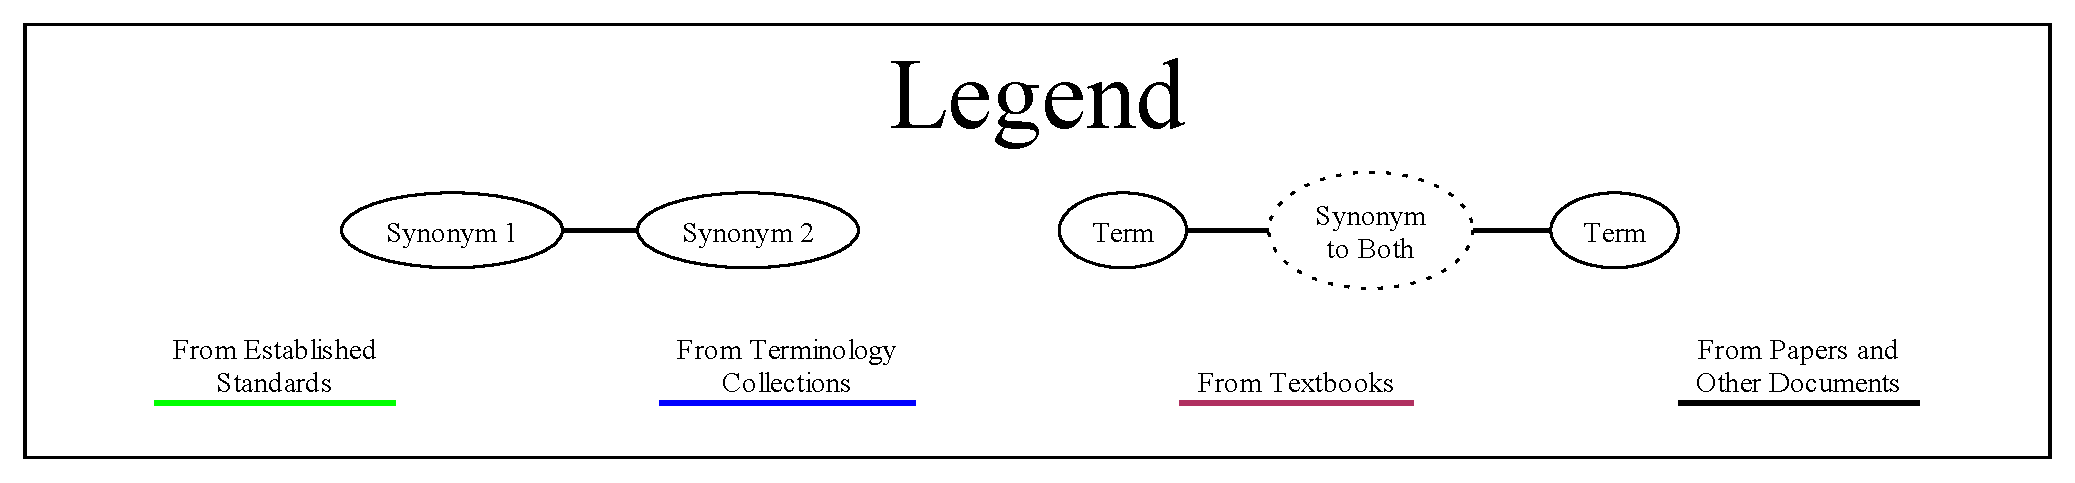
\includegraphics[width=\textwidth]{assets/graphs/manual/expSynLegend.pdf}
        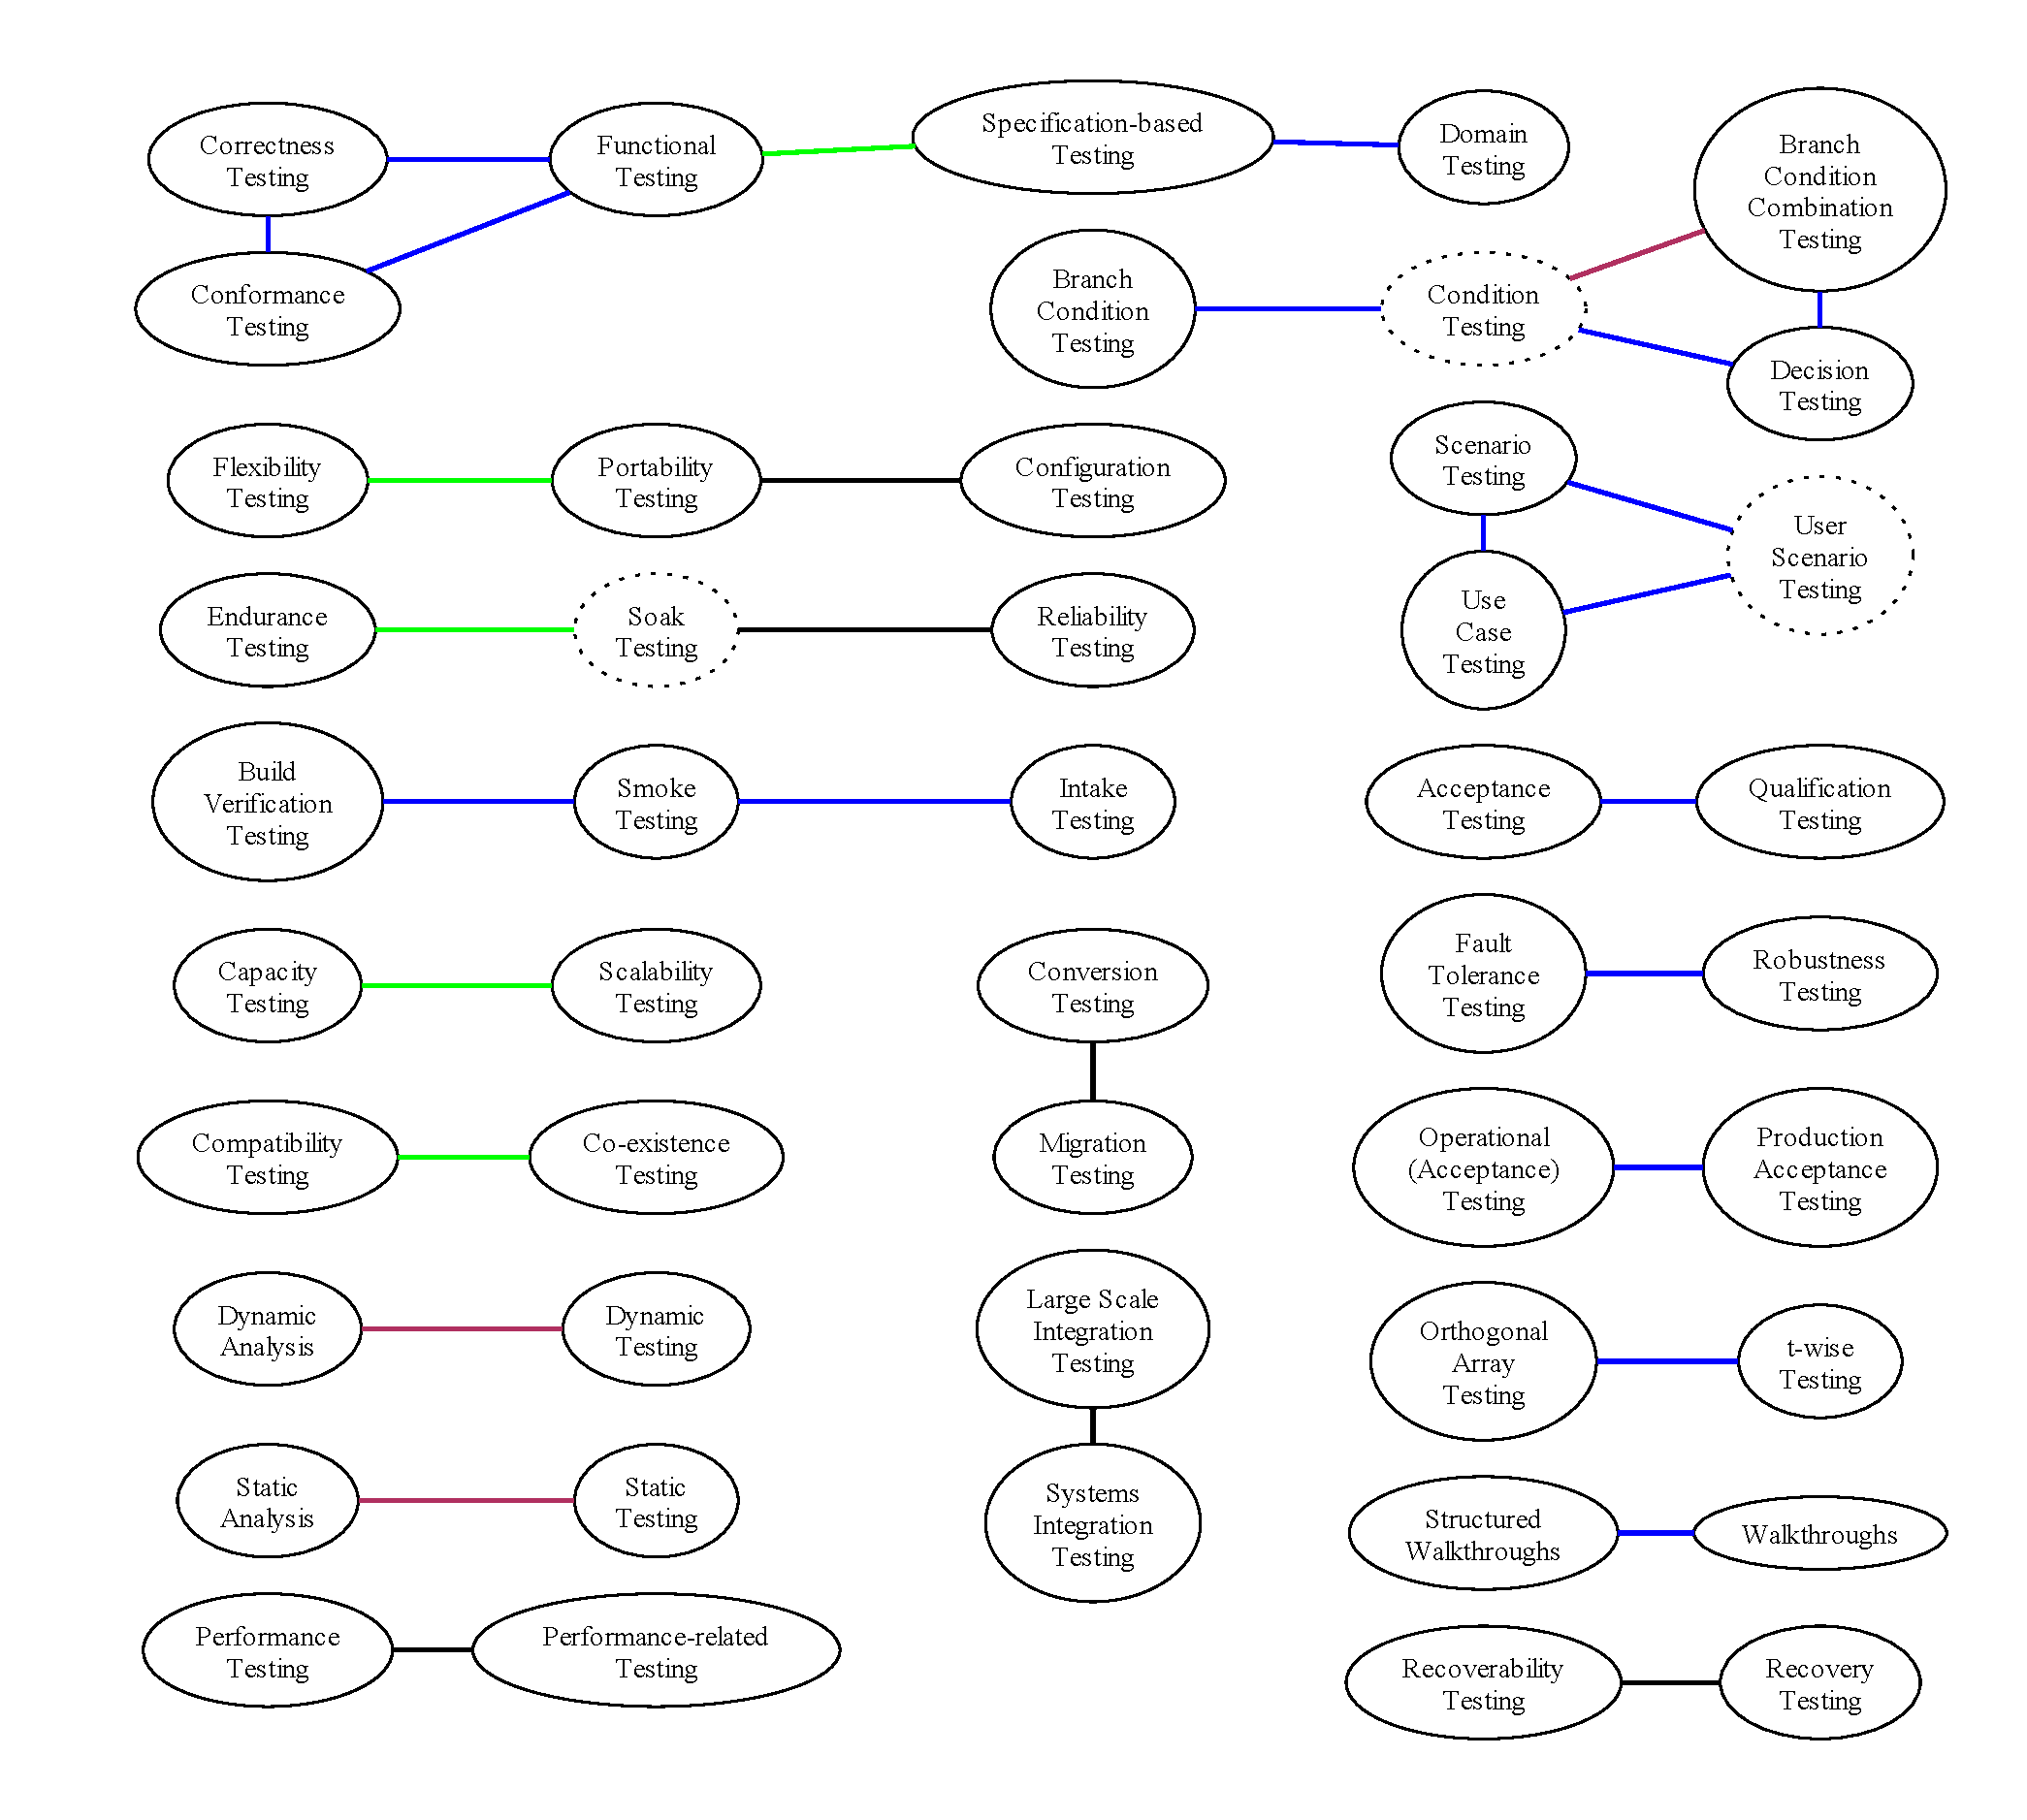
\includegraphics[width=\textwidth]{assets/graphs/manual/expSynGraph.pdf}
        % \vspace{-7mm}
        \caption{Synonym relations given explicitly by the literature.}
        \label{fig:expSynGraph}
    \end{figure}

    \phantomsection{}\label{graphExplicit}
    Since we also track the ``explicitness'' of information
    (see \Cref{explicitness}), we can represent explicit
    \emph{and} implicit relations without double counting them during the
    analysis in \Cref{flaw-analysis}. If a relation is both explicit
    \emph{and} implicit, we only include the implicit relation in the graph
    if its source is more ``credible'' (see \Cref{cred}).
    For example, only the explicit synonym relation between E and F
    from \Cref{tab:exampleGlossary} appears in \Cref{fig:synExampleGraph}.
    Implicit approaches and relations are denoted by dashed lines, as shown
    in \Cref{fig:exampleGraph,fig:synExampleGraph}; explicit approaches are
    \emph{always} denoted by solid lines, even if they are also implicit.
    We can also generate ``explicit'' versions of these graphs that exclude
    implicit approaches and relations; for example, \Cref{fig:expExampleGraph}
    is the explicit version of \Cref{fig:exampleGraph}, and
    \Cref{fig:expSynGraph} likewise only contains explicit approaches and
    synonym relations.

\fi
Since these graphs tend to be large, it is useful to focus on specific
subsets of them. \ifnotpaper For each approach category (see
    \Cref{cats-def}), we generate a graph restricted to its approaches
    and the relations between them. We also generate a graph of all static
    approaches along with the relations between them \emph{and} between a
    static approach and a dynamic approach. We generate this static-focused
    graph because static testing is sometimes considered to be a separate
    approach category (see \flawref{static-test-flaw}), but we include the
    relations with dynamic approaches since they are our primary focus
    (see \Cref{static-test}). We color all dynamic approach nodes in these
    graphs grey, as in \Cref{fig:staticExampleGraph}, to distinguish them,
    and include this in the legend of \Cref{fig:exampleGraphs} for convenience.
    If we assume that the approaches in \Crefrange{fig:exampleGraph}
    {fig:parSynExampleGraph} are all static, then this portion of the legend
    applies to the entirety of \Cref{fig:exampleGraphs}; otherwise, it only
    applies to \Cref{fig:staticExampleGraph}.\qtodo{Does this make sense?}

    We can also generate more specific subsets of these graphs
\else We can generate more focused graphs \fi from a given subset of
approaches, such as \ifnotpaper\else those in a selected approach category
    (see \Cref{cats-def}) or \fi those pertaining to recovery or
scability\ifnotpaper. These areas are of particular note as we discuss their
flaws in their own sections (\Cref{recov-flaw,scal-flaw}, respectively).
We generate graphs of just these subsets of software testing to help visualize
the relations between these approaches, given \else; the latter are shown \fi
in \Cref{fig:rec-graph-current,fig:scal-graph-current}, respectively. By
specifying sets of approaches and relations to add or remove, we can then
update these generated graphs based on our recommendations; applying those
given in \Cref{rec-test-rec,,scal-test-rec,,\ifnotpaper\else perf-test-rec\fi}
results in the updated graphs in \Cref{fig:rec-graph-proposed,,%
    fig:scal-graph-proposed,,\ifnotpaper\else fig:perf-graph\fi}, respectively.
We color any added approaches or relations orange to distinguish them.
% \ifnotpaper
Recommendations can also be inherited; for example, we generate
\Cref{fig:perf-graph} based on the modifications we apply to
\Cref{fig:rec-graph-proposed,fig:scal-graph-proposed} and
other changes from \Cref{perf-test-rec}.
% \fi

\ifnotpaper
    \subsection{Flaw Analysis}
\label{flaw-analysis}

In addition to analyzing specific flaws, it is also useful to examine them at
a higher level. We automate subsets of this task where applicable
(\Cref{auto-flaw-analysis}) and augment the remaining manual portion with
automated tools (\Cref{aug-flaw-analysis}). This gives us an overview of:
\begin{itemize}
    \item how many flaws there are,
    \item how responsible each source tier (see \Cref{sources}) is for these flaws,
    \item how obvious (or ``rigid''; see \Cref{rigidity}) these flaws are,
    \item how these flaws present themselves (see \Cref{flawMnfsts}), and
    \item in which knowledge domains these flaws occur (see \Cref{flawDmns}).
\end{itemize}

To understand where flaws exist in the literature, we group them based on the
source tier(s) responsible for them. Each flaw is then counted \emph{once} per
source tier if it appears within it \emph{and/or} between it and a more
``credible'' tier\footnote{If an inconsistency occurs between two source tiers
    and the more credible one is \emph{incorrect}, we instead count it as an
    inconsistency between it and ground truth, as described in
    \Cref{lower-ground-truth}.} (see \Cref{cred,sources}). This avoids
counting the same flaw
more than once for a given source tier\thesisissueref{83}, which would give the
number of \emph{occurrences} of all flaws instead of the more useful number of
flaws \emph{themselves}. The exception to this is \Cref{fig:flawBars}, which
counts the following sources of flaws separately:
\begin{enumerate}
    \item those that appear once in (or consistently throughout) a document
          (i.e., are ``self-contained'')\thesisissueref{137,138},
    \item those between two parts of a single document
          (i.e., internal conflicts)\thesisissueref{137,138},
    \item those between documents with the same set of authors, which includes
          \begin{enumerate}
              \item the various combinations of ISO, the \acf{iec}, and IEEE
                    shown in \Cref{fig:ieeeSourceSets} and
              \item the different versions of the \acfp{swebok}, which have
                    different editors \citep{SWEBOK2024,SWEBOK2014} but are
                    written by the same organization: the IEEE Computer Society
                    (\citealp{AboutSWEBOK}; see \Cref{metas}), and
          \end{enumerate}
    \item those within a single source tier.
\end{enumerate}
As before, these are not double counted, meaning that the maximum number of
counted flaws possible within a \emph{single} source tier in
\Cref{fig:flawBars} is four (one for each type). This only occurs if
there is an example of each flaw source that is \emph{not} ignored to
avoid double counting; for example, while a single flaw within a single
document would technically fulfill all four criteria, it would only be counted
once.

\begin{figure}[bt!]
    \centering
    \begin{tikzpicture}
        \def\radius{3.6cm}
        \def\spread{1.5}
        \def\offset{\spread*1.6}

        \draw (-\spread, 0) circle (\radius);
        \draw ( \spread, 0) circle (\radius);
        \draw (0, -\offset) circle (\radius);

        \node[above] at (-\offset,        \radius) {ISO};
        \node[above] at ( \offset,        \radius) {IEC};
        \node[above] at (0, -\offset-1.85*\radius) {IEEE};

        % ALL
        \node[above] at (0, -\spread-0.5) {\parbox{3.7cm}{\centering
                \citealp{IEEE2022,IEEE2021,IEEE2019a,IEEE2019b,IEEE2017,
                    IEEE2016,IEEE2013,IEEE2010}}};
        % ISO/IEC
        \node[above] at (0, 0.325*\radius) {\parbox{2.8cm}{\centering
                \citealp{ISO_IEC2023a,ISO_IEC2023b,ISO_IEC2018,ISO_IEC2015,ISO_IEC2011}}};
        % ISO/IEEE
        \node[above] at ( \offset, -\offset) {---};
        % IEC/IEEE
        \node[above] at (-\offset, -\offset) {---};

        % ISO
        \node[above] at (-1.4*\offset, 0.25) {\parbox{2cm}{\centering
                \citealp{ISO2022,ISO2015}}};
        % IEC
        \node[above] at ( 1.4*\offset, 0.25) {---};
        % IEEE
        \node[above] at (0, -\spread-1.4*\radius) {\citealp{IEEE2012}};

    \end{tikzpicture}
    \caption{The sets of authors of established standards (see \Cref{stds}).}
    \label{fig:ieeeSourceSets}
\end{figure}

\phantomsection{}
\label{flaw-analysis-example}
As an example of this process, consider \flawref{level-phase-syns}, where an
IEEE standard has an internal flaw, and an inconsistency with two other IEEE
standards, and an inconsistency with a textbook. This adds one to the following
rows of \Cref{tab:flawMnfsts,tab:flawDmns} in the relevant column for a total
of two counted flaws:

\begin{itemize}
    \item \textbf{\stds{}}: this flaw occurs:
          \begin{enumerate}
              \item within one standard and
              \item between three standards (with the same set of authors).
          \end{enumerate}
          This increments the count by just one to avoid double counting and
          would do so even if only one of the above conditions was true. A more
          nuanced breakdown of flaws that identifies those within a
          singular document and those between documents by the same author is
          given in \Cref{fig:flawBars} and explained in more detail in
          \Cref{aug-flaw-analysis}; this view counts three total flaws here.
    \item \textbf{\texts{}}: this flaw occurs between a source in this tier and
          a ``more credible'' one (the IEEE standards; see \Cref{cred}).
          % \item \textbf{\papers{}}: this flaw occurs between a source in this tier
          %       and a ``more credible'' one. Even though there are two sources in this
          %       tier \emph{and} two ``more credible'' tier involved, this increments
          %       the count by just one to avoid double counting.
\end{itemize}

\subsubsection{Automated Flaw Analysis}
\label{auto-flaw-analysis}

As outlined in \Cref{graph-gen}, we automatically detect test approaches that
share a synonym (\hyperref[case-three]{Case 3} in \Cref{graph-gen}) to generate
our graphs. These relations are significant because they are potential flaws.
They arise from glossary entries such as those in \Cref{tab:synExampleGlossary}
which we automatically detect, format, and present in
\Cref{multiSyns,infMultiSyns}. The next logical step is to detect other classes
of flaws.\phantomsection{}\label{selfCycles}
The self-referential definitions in \Cref{selfPars} (defined as
$\left\{(x, y) \in P \mid x = y\right\}$) are also trivial to automate by
looking for lines in the
generated \LaTeX{} files that start with \texttt{I~->~I}, where \texttt{I}
is the label used for a test approach node in these graphs. This process
results in output similar to \Cref{fig:selfExampleGraph}. We use a similar
process to detect pairs of approaches with a synonym relation \emph{and} a
parent-child relation, defined as
$\left\{(x, y) \in P \mid \{x, y\} \in S\right\}$ and given in
\Cref{tab:parSyns,infParSyns}. To accomplish this, we build a dictionary of
each term's synonyms to evaluate which synonym relations are notable enough
to include in the graph, and then check these mappings to see if one appears
as a parent of the other. For example, if \texttt{J} and \texttt{K} are
synonyms, a generated \LaTeX{} file with a parent line starting with
\texttt{J~->~K} would result in these approaches being graphed as shown in
\Cref{fig:parSynExampleGraph}.

While just counting the total number of flaws (found automatically \emph{or}
manually) is trivial, tracking
the source(s) of these flaws is more useful, albeit more involved. Since
we consistently track the appropriate citations for each piece of information
we record (see \Cref{tab:exampleGlossary,tab:synExampleGlossary} for examples
of how these citations are formatted in the glossaries), we can use them to
identify the offending source tier(s). This comes with the added benefit that
we can format these citations to use with \LaTeX{}'s citation commands in this
\docType{}.

We compare the authors and years of each source involved with a given flaw
to determine if it manifests within a single document and/or between documents
with the same set of authors. Then, we group these sources into their tiers
\seeSrcCode{82167b7}{scripts/flawCounter.py}{63}{80}.
% done by the function in \Cref{lst:getSrcCat}, since each source tier
% outlined in \Cref{sources} is comprised of a small number of authors (with the
% exception of papers and other documents; see \Cref{papers}).
We then distill these lists of sources down to sets of tiers and compare them
against each other to determine how many times a given flaw manifests between
source tiers. This determines which row(s) of \Cref{tab:flawMnfsts,tab:flawDmns}
and which bar(s) of \Cref{fig:flawBars} that the given flaw should count toward.
We describe this process in more detail in \Cref{aug-flaw-analysis}.

\phantomsection{}
\label{auto-flaw-analysis-rigidity}
Alongside this citation information, we include keywords so we can assess how
``rigid'' a piece of information is (see \Cref{rigidity}). This is useful when
counting flaws, since they can be both explicit and implicit but should not be
double counted as both\thesisissueref{83}! When counting flaws in
\Cref{tab:flawMnfsts,tab:flawDmns}, each one is
counted only for its most ``rigid'' manifestation (i.e., it will only increment
a value in the ``Implicit'' column if it is \emph{not} also explicit),
similarly to how we generate graphs (see \Cref{graphRigid}).

\subsubsection{Augmented Flaw Analysis}
\label{aug-flaw-analysis}
While we can detect some subsets of flaws automatically by analyzing
\ourApproachGlossary, most are too complex and need to be tracked manually. We
record these more detailed flaws as \LaTeX{} enumeration items along with
comments that we can parse automatically, allowing us to analyze them more
broadly. We also add these comments to flaws we detect automatically before
generating the corresponding \LaTeX{} file to ensure these flaws also get
analyzed. These comments have the following format:
\begin{displayquote}
    \texttt{\% Flaw count (MNFST, DMN): \{A1\} \{A2\} \dots{} | \{B1\} % \{B2\}
        \dots{} | \{C1\} \dots}
\end{displayquote}
\texttt{MNFST} and \texttt{DMN} are placeholders for the ``keys'' given in
\Cref{tab:flawMnfstDefs,tab:flawDmnDefs}, respectively, that we use to track a
flaw's manifestation(s) and domain(s) (defined in \Cref{flaw-def}). We omit
these keys from constructed examples of these comments without associated flaws
throughout this chapter for brevity. Finally, \texttt{A1}, \texttt{A2}, % \texttt{B2},
\texttt{B1}, and \texttt{C1} are each placeholders for a source involved in
this example flaw; in general, there can be arbitrarily many. We represent each
source by its \BibTeX{} key, and wrap each one in curly braces (with the
exception of the \acs{istqb} glossary due to its use of custom commands via
\macro{citealias}) to mimic \LaTeX{}'s citation commands for ease of parsing.
We then separate each ``group'' of sources with a pipe symbol (\texttt{|}) so
we can compare each pair of groups; in general, a flaw can have any number of
groups of sources.

We make a distinction between ``self-contained'' flaws and ``internal'' flaws.
Self-contained flaws are those that manifest by comparing a document to a
source of ground truth. Sometimes, these do not require an explicit comparison;
for example, omissions (listed in \Cref{miss}) often fall into this category,
since the lack of information is contained within a single source and does not
need to be cross-checked against a source of ground truth. If only one group of
sources is present in a flaw's comment, such as the first line below, we
consider it to be a self-contained flaw. On the other hand, internal flaws
arise when a document disagrees with itself by containing two conflicting
pieces of information; this includes many contradictions and overlaps (listed
in \Cref{contra,over}, respectively). These can even occur on the same page,
such as when a source gives an acronym to two distinct terms
(see \flawref{cat-acro,hil-acro})! If a
source appears in multiple groups in a flaw's comment, we consider it to
be an internal flaw. The second line is a standard example of this, while the
third is more complex; in this case, source Y agrees with only one of the
conflicting sources of information in X.
\begin{displayquote}
    \texttt{\% Flaw count: \{X\}\\\% Flaw count: \{X\} | \{X\}\\
        \% Flaw count: \{X\} | \{X\} \{Y\}}
\end{displayquote}
We do not double count flaws that reappear when comparing between pairs of
groups; this means the following line adds an inconsistency between X and Z
\emph{and} between Y and Z \emph{without} double counting the former.
\begin{displayquote}
    \texttt{\% Flaw count: \{X\} | \{X\} \{Y\} | \{Z\}}
\end{displayquote}
To give a more complete example, we track \flawref{level-phase-syns} with the
following comment line:\utd{}
\begin{displayquote}
    \texttt{\% Flaw count (OVER, SYNS): \{IEEE2017\} \{IEEE2013\} | \{IEEE2022\}
        \displayNL{} \{IEEE2017\} \{Perry2006\}}
\end{displayquote}%
We parse this as the example given in \Cref{flaw-analysis-example}. Since
\texttt{IEEE2022}, \texttt{IEEE2017}, and \texttt{IEEE2013} are all written by
the same standards
organizations (\begin{NoHyper}\citeauthor{IEEE2022}\end{NoHyper}), we count
this as an inconsistency between documents with the same set of authors in
\Cref{fig:flawBars}, but only once to avoid double counting.

We can also specify the rigidity (see \Cref{rigidity}) of a flaw by inserting
the phrase ``implied by'' after the sources of explicit information and before
those of implicit information. This information is parsed following the same
rules described in \Cref{auto-flaw-analysis-rigidity} for automatically
detected flaws. Note that we only count implicit flaws if there is not an
equivalent explicit flaw, as we do when generating graphs (\Cref{graphRigid}).
\begin{displayquote}
    \texttt{\% Flaw count (CONTRA, DEFS): \{IEEE2021\} \{IEEE2017\} |
        \displayNL \{vanVliet2000\} implied by \{IEEE2021\}}
\end{displayquote}
For example, the above comment line\utd{} from \flawref{c-use-def} indicates
that the flaws given below are present. The third flaw only affects
\Cref{fig:flawBars} due to its more nuanced breakdown of the
sources of flaws. The rest increment their corresponding count in
\Cref{fig:flawBars,tab:flawMnfsts,tab:flawDmns} by only one:
\begin{itemize}
    \item an explicit inconsistency between a textbook and a standard,
    \item an implicit flaw within a single document, and
    \item an implicit inconsistency between documents with the same set of
          authors (\begin{NoHyper}\citeauthor{IEEE2022}\end{NoHyper}).
\end{itemize}

\phantomsection{}\label{lower-ground-truth}
Occasionally, we use a source from a lower tier as the ``ground truth'' for a
flaw. For example, \tolTestFlaw*{} This flaw is supported
by additional papers found via a miniature literature review (described in
\Cref{undef-terms}) from a lower source tier than \citep{Firesmith2015}
(which is a terminology collection; see \Cref{sources}). However, this flaw
is really based in \citep{Firesmith2015} and not in these
additional papers, but this would be counted as a flaw in these papers if they
were included as detailed above. Therefore, we document these ``ground
truth'' sources separately to track them for traceability without incorrectly
counting flaws, such as the following for this specific example
(\flawref{ground-truth}):
\begin{displayquote}
    \texttt{\% Flaw count (WRONG, LABELS): \{Firesmith2015\}\\
        \% Ground truth: \{LiuEtAl2023\} \{MorgunEtAl1999\} \{HolleyEtAl1996\}
        \displayNL \{HoweAndJohnson1995\}}
\end{displayquote}

\subsection[LaTeX Commands]{\LaTeX{} Commands}\label{macros}
To improve maintainability, traceability, and reproducibility, we define
helper commands (also called ``macros'') for content that is prone to change
or used in multiple places. For example, we use Python scripts to calculate
values based on our glossaries and save them to files to be assigned to
corresponding \LaTeX{} macros. We use these throughout our documents instead of
manually updating these constantly changing values, which is prone to error.
\Cref{tab:macrosCalc} lists these macros, along with their current values and
descriptions of what they represent. Our Python scripts convert numbers to
their textual equivalents when necessary to follow IEEE guidelines.

\begin{longtblr}[
    note{a} = {Calculated in \LaTeX{} from source tier lists; see \Cref{text-macros}.},
    note{b} = {Alias for \texttt{\textbackslash totalFlawDmnBrkdwn\{13\}}; see \Cref{flawCounts}.},
    note{c} = {These macros are defined as counters to allow them to be used in
            calculations within \LaTeX{} (such as in \Cref{undef-terms,fig:undefPies}).},
    caption = {\LaTeX{} macros for calculated values.},
    label = {tab:macrosCalc}
    ]{
    colspec={|X[0.3,l,m]X[0.5,c,m]X[0.2,c,m]|},
    width = \linewidth, rowhead = 1
    }
    \hline
    \thead{Macro}                                   & \thead{What it Counts}        & \thead{Value}    \\
    \hline
    \macro{approachCount}                           & Identified test approaches    & \approachCount{} \\
    \macro{qualityCount}                            & Identified software qualities & \qualityCount{}  \\
    \macro{srcCount}\TblrNote{a}                    & Sources used in glossaries    & \srcCount{}      \\
    \macro{flawCount}\TblrNote{b}                   & Identified flaws              & \flawCount{}     \\
    \hline
    \macro{TotalBefore}\TblrNote{c}                 & Test approaches identified
    before process in \Cref{undef-terms}            & \the\TotalBefore{}                               \\
    \macro{UndefBefore}\TblrNote{c}                 & Undefined test approaches
    identified before process in \Cref{undef-terms} & \the\UndefBefore{}                               \\
    \macro{TotalAfter}\TblrNote{c}                  & Test approaches identified
    after process in \Cref{undef-terms}             & \the\TotalAfter{}                                \\
    \macro{UndefAfter}\TblrNote{c}                  & Undefined test approaches
    identified after process in \Cref{undef-terms}  & \the\UndefAfter{}                                \\
    \hline
    \macro{multiSynCount}                           & Terms given as synonyms for
    multiple discrete terms                         & \multiSynCount{}                                 \\
    \macro{parSynCount}                             & Pairs of test approaches
    with a child-parent \emph{and} synonym relation & \parSynCount{}                                   \\
    \macro{selfCycleCount}                          & Test approaches that are
    a parent of themselves                          & \selfCycleCount{}                                \\
    \hline
\end{longtblr}


\phantomsection{}\label{flawCounts}
Additionally, we count flaws based on their manifestation and domain, rigidity,
and source tier (defined in \Cref{flaw-def,rigidity,sources}, respectively).
For each source tier, we create two files that each include both levels of
rigidity: one for manifestations and one for domains. For example, flaws in
standards are saved to \texttt{build/stdFlawMnfstBrkdwn.tex} by manifestation%
% and \texttt{build/stdFlawDmnBrkdwn.tex} for domains
. We then assign these data to macros (such as \macro{stdFlawMnfstBrkdwn}) to
populate \Cref{tab:flawMnfsts,tab:flawDmns}. For example, we access the number
of explicit and implicit mistakes in standards by using
\macro[1]{stdFlawMnfstBrkdwn} and \macro[2]{stdFlawMnfstBrkdwn}, respectively.
We follow a similar process for tracking the total numbers of flaws; this
includes \macro[13]{totalFlawMnfstBrkdwn} and \macro[13]{totalFlawDmnBrkdwn}
which are identical and track the total number of identified flaws.

\phantomsection{}\label{text-macros}
Just as with calculated values, it is important that repeated text is updated
consistently, which we accomplish by defining more macros. Some of these are
generated by Python scripts in a similar fashion to calculated values, such as
those for flaw manifestations and domains in \Cref{tab:macrosSections} and the
lists of sources in each source tier. The latter are built by extracting all
sources cited in our three glossaries, categorizing, sorting, and formatting
them (including handling edge cases), and saving them to a file. These are then
assigned to \macro{stdSources}, \macro{metaSources}, \macro{textSources}, and
\macro{paperSources} and include:
\begin{enumerate}
    \item the source tier's name,
    \item the list of sources in the tier, and
    \item the number of sources in the tier.
\end{enumerate}
These are accessed by passing in the corresponding number in the above
enumeration (e.g., \macro[2]{paperSources}). We use the first value for the
subheadings in \Cref{sources}, the first two for \Cref{app-src-tiers} and the
third to build \Cref{fig:sourceSummary} and calculate \macro{srcCount}
(see \Cref{tab:macrosCalc}).
% We also define macros for well-defined sections in \Cref{tab:macrosSections}.

\afterpage{
    \begin{landscape}
        \begin{longtblr}[
    note{a} = {Defined in \Cref{mnfst-def}; we also define starred versions,
            such as \macro{wrong*} (\wrong*{}), that use the singular noun for
            use in \Cref{tab:flawMnfstDefs}.},
    note{b} = {Defined in \Cref{dmn-def}; we only include domains with their
            own section.},
    % we also define starred versions,
    % such as \macro{cats*} (\cats*{}), that use the singular noun.
    note{c} = {Defined in \Cref{source-tiers}.},
    note{d} = {We overwrite the primitive \TeX{} command \macro{over}
            % Source: https://tex.stackexchange.com/a/73825/192195
            since we do not otherwise use it.},
    % note{e} = {We define a starred version, \macro{papers*} (\papers*{}), to shorten the
    %         display name for use in tables.},
    caption = {\LaTeX{} macros for referencing well-defined sections.},
    label = {tab:macrosSections}
    ]{
    colspec={|Q[1.75cm,c,m]|Q[l,m]Q[r,m]|Q[l,m]Q[r,m]|Q[l,m]Q[r,m]|},
    row{1} = {halign=c},
    width = \textwidth, rowhead = 1
    }
    \hline
                     & \SetCell[c=2]{c} \thead{Flaw Manifestations\TblrNote{a}}  &             & \SetCell[c=2]{c} \thead{Flaw Domains\TblrNote{b}} &           & \SetCell[c=2]{c} \thead{Source Tiers\TblrNote{c}} &              \\
    \hline
    \SetCell[r=6]{c} \textbf{Macros                                                                                                                                                                                               \\
    (Values)}        & \macro{wrong}                                             & (\wrong{})  & \macro{cats}                                      & (\cats{}) & \macro{stds}                                      & (\stds{})    \\
                     & \macro{miss}                                              & (\miss{})   & \macro{syns}                                      & (\syns{}) & \macro{metas}                                     & (\metas{})   \\
                     & \macro{contra}                                            & (\contra{}) & \macro{pars}                                      & (\pars{}) & \macro{texts}                                     & (\texts{})   \\
                     & \macro{ambi}                                              & (\ambi{})   &                                                   &           & \macro{papers}                                    & (\papers{})  \\ %\TblrNote{e}                                              \\
                     & \macro{over}\TblrNote{d}                                  & (\over{})   &                                                   &           & \macro{papers*}                                   & (\papers*{}) \\
                     & \macro{redun}                                             & (\redun{})  &                                                   &           &                                                                  \\
    \hline
    \textbf{Used In} & \SetCell[c=2]{c} {\Cref{tab:flawMnfstDefs,tab:flawMnfsts}
        % \\ (in both thesis and paper)
    }                &
                     & \SetCell[c=2]{c} {\Cref{tab:flawDmnDefs,tab:flawDmns}
        % \\ (in both thesis and paper)
    }                &                                                           &
    \SetCell[c=2]{c} {
    \Cref{fig:sourceSummary,fig:flawBars,fig:flawBarsSummary,fig:normFlawBarsSummary}                                                                                                                                             \\
        \Cref{tab:flawMnfsts,tab:flawDmns}
        % \\ \Cref{flaw-analysis-example} (only \macro{stds} and \macro{texts})
    }                &                                                                                                                                                                                                            \\
    \hline
\end{longtblr}

    \end{landscape}}

However, we create most of these macros for reused text manually when we first
notice the reuse, including the source tier macros in \Cref{tab:macrosSections}.
Some of these macros account for context-specific formatting depending on how
they are used, such as capitalization. These tend to be less well-defined,
since they arise naturally from the writing process, so we omit these details
from the manually created text macros in \Cref{tab:macrosText}, which are
grouped based on the type of information they contain.

% With help from https://tex.stackexchange.com/a/40468/192195, https://tex.stackexchange.com/a/245663/192195, and Copliot
\newcommand\macroType[2]{\multirow[b]{#1}{*}{\adjustbox{minipage=\the\dimexpr 0.3cm * #1 \relax,rotate=90}{#2}}}
% \newcommand\macroType[2]{\multirow[c]{#1}{*}{\rotatebox[origin=c]{90}{#2}}}

\begin{longtblr}[
    note{a} = {Defined in \Cref{flaw-def}.},
    note{b} = {See \Cref{tab:macrosSections} for more details on how we use
            \macro{redunNote} alongside \macro{redun}.},
    caption = {\LaTeX{} macros for reused text.},
    label = {tab:macrosText}
    ]{
    colspec={|Q[c,m]Q[l,m]X[l,m]|},
    row{1} = {halign=c},
    width = \textwidth, rowhead = 1
    }
    \hline
    \thead{Type}             & \thead{Macro}               & \thead{Used in}                                             \\*
    \hline
    \macroType{12}{Flaws\TblrNote{a}}
                             & \macro{bugPattonFlaw}       & \Cref{intro} and \flawref{bug-patton}                       \\*
                             & \macro{alphaFlaw}           & \Cref{intro} and \flawref{alpha-def}                        \\*
                             & \macro{loadFlaw}            & \Cref{intro} and \flawref{load-def}                         \\*
                             & \macro{expBasedCatMain}     & \Cref{intro,multiCats}                                      \\*
                             & \macro{tourFlaw}            & \Cref{intro,flaws} and \flawref{tour-def}                   \\*
                             & \macro{redBoxFlaw}          & \Cref{explicitness,wrong} and \flawref{dubious-red-box-syn} \\*
                             & \macro{perfAsFamily}        & \Cref{method-family,classFamilyFlaw}                        \\*
                             & \macro{tolTestFlaw}         & \Cref{less-cred-assert,wrong} and \flawref{assert-truth}    \\*
                             & \macro{accelTolTest}        & \macro{tolTestFlaw} and \Cref{hard-test}                    \\*
                             & \macro{errorGuessFlaw}      & \Cref{wrong} and \flawref{error-guess}                      \\*
                             & \macro{parSheetTestFlaw}    & \Cref{wrong} and \flawref{par-sheet-test}                   \\*
                             & \macro{perfSecParFlaw}      & \flawref{perf-sec-par} and paper version of \Cref{pars}     \\
    \hline
    \macroType{7}{Footnotes} & \macro{ftrnote}             & \SetCell[r=3]{l} Thesis (automated) and paper (manual)
    versions of \Cref{tab:parSyns}                                                                                       \\*
                             & \macro{specfn}              &                                                             \\*
                             & \macro{ucstn}               &                                                             \\*
    \cline{2-3}              & \macro{redunNote}           & \macro{redun} and \Cref{tab:flawMnfstDefs}\TblrNote{b}      \\*
    \cline{2-3}              & \macro{notDefDistinctIEEE}  & \flawref{static-test-flaw} and \Cref{exist-tax}             \\*
                             & \macro{gerrardDistinctIEEE} & \Cref{tab:otherCategorizations} and
    \flawref{gerrard-distinct}                                                                                           \\*
                             & \macro{distinctIEEE}        & \macro{gerrardDistinctIEEE}, \macro{notDefDistinctIEEE},
    and \Cref{method-family,classFamilyFlaw}                                                                             \\
    \hline
    \macroType{3}{Links}     & \macro{ourApproachGlossary} &
    \Cref{tab:approachGlossaryExcerpt,explicitness,record-terms,imp-info,app-rel-vis,%
    auto-flaw-analysis,aug-flaw-analysis,oat-test-rec}                                                                   \\*
                             & \macro{seeSrcCode}          & \Cref{app-rel-vis,auto-flaw-analysis}                       \\*
    % paper-macros
                             & \macro{recFigs}             & \Cref{flaws,recs}                                           \\
    \hline
    \macroType{3}{RQs}       & \macro{rqatext}             & \SetCell[r=3]{l} \Cref{intro} and seminar slides            \\*
                             & \macro{rqbtext}             &                                                             \\*
                             & \macro{rqctext}             &                                                             \\
    \hline
    \macroType{12}{Misc.}    & \macro{supersAck}           & \nameref{acknowledgements} and seminar slides               \\*
                             & \macro{supers}              & \nameref{decl_aca_ach} and \macro{supersAck}                \\*
                             & \macro{highLvlScope}        & \Cref{scope-overview,stds}                                  \\*
                             & \macro{defRel}              & \Cref{syn-rels,par-chd-rels}                                \\*
                             & \macro{defLabelDistinct}    & \Cref{label-flaw-def,labels}                                \\*
                             & \macro{oneSrcDistinct}      & \Cref{one-src-flaws,aug-flaw-analysis}                      \\*
                             & \macro{approachFields}      & \Cref{explicitness,record-terms}                            \\*
                             & \macro{impKeywords}         & \Cref{explicitness,imp-info}                                \\*
                             & \macro{orthTestIntro}       & \Cref{infers,orth-test}                                     \\*
                             & \macro{listAllSrcs}         & \Cref{source-tiers,ident-sources}                           \\*
                             & \macro{addTextEx}           & \Cref{texts,ident-sources}                                  \\*
                             & \macro{displayNL}           &
    \Cref{app-rel-vis,aug-flaw-analysis}                                                                                 \\
    % paper-macros,tab:macrosPaper
    \hline
\end{longtblr}


\phantomsection{}\label{paper-macros}
In addition to this thesis, we also prepare a conference paper based on our
research. While we can reuse most content without modifying it, we need to
address the formatting differences between the two document types.
In general, we use the conditional \texttt{\textbackslash ifnotpaper} to allow
for manual distinctions between the two documents' formats using this basic
template:
\begin{displayquote}
    \texttt{\textbackslash ifnotpaper <thesis code> \textbackslash else <paper code> \textbackslash fi}
\end{displayquote}
We define the macros given in \Cref{tab:macrosPaper} for recurring edge cases
between formatting requirements for these document types, presented along with
example usages and renderings. Since this document is the thesis, we have to
hardcode some of the paper renderings, so they may not be perfectly accurate.

\def\refHelperEx{\refHelper \ifnotpaper \citet{IEEE2022}
    \else \defcitealias{IEEE2022}{16}[\citetalias{IEEE2022}]
    \fi \multiAuthHelper{form} the basis of this \docType{}.}

\begin{longtblr}[
    note{a} = {Section omitted for brevity.},
    caption = {\LaTeX{} macros for handling formatting differences between thesis and paper.},
    label = {tab:macrosPaper}
    ]{
    colspec={|Q[c,m]|X[l,m]|},
    column{1} = {font=\bfseries},
    width = \textwidth, rowhead = 1
    }
    \hline
    \thead{Context} & \thead{Displayed as}                                                \\
    \hline
    Code            & {\texttt{\macro{refHelper} \macro[IEEE2022]{citet}\
    \macro[form]{multiAuthHelper}} \displayNL\texttt{the basis of this \macro{docType}.}} \\*
    Thesis          & \refHelperEx{}                                                      \\*
    Paper           & {\notpaperfalse \refHelperEx{}}                                     \\
    \hline
    Code            & \macro[cat-acro]{flawref}                                           \\*
    Thesis          & \flawref{cat-acro}                                                  \\*
    Paper           & Section \hyperref[cat-acro]{III-B2}                                 \\
    \hline
    Code            & \macro{redun}                                                       \\*
    Thesis          & \redun{}                                                            \\*
    Paper           & Redundancies\TblrNote{a}                                            \\
    \hline
\end{longtblr}


The most common difference between the two document styles is how citations are
displayed. We use the \texttt{natbib} package for our thesis, but the IEEE
guidelines for paper submissions suggest the use of \texttt{cite}
\citep[p.~8]{Shell2015a}. For simplicity, we define aliases so we can reuse
text that includes a single citation
\seeSrcCode{0a2dcdf}{paper_preamble.tex}{19}{60}. However, text that
cites multiple sources requires more work to be reused and has to be done so
manually, since the \texttt{natbib} package groups multiple citations within a
single set of parentheses while the \texttt{cite} package keeps them separate
inside their own set of square brackets.

For example, in \Cref{nonIEEE-sources}, we provide a list of non-IEEE sources
that support a claim made by the IEEE. Since we sort sources based on
credibility (defined in \Cref{cred}) and then by publication year, the
relevant thesis code is given below. (We use ``\texttt{\textbackslash =/}'',
etc. from the \texttt{extdash} package for non-breaking dashes.)
\begin{displayquote}
    \texttt{(\textbackslash citealp[pp.\textasciitilde 5\textbackslash =/6 to 5\textbackslash =/7]\{SWEBOK2024\};
        \displayNL \textbackslash citealpISTQB\{\};
        \textbackslash citealp[pp.\textasciitilde 807\textbackslash ==808]\{Perry2006\};
        \displayNL \textbackslash citealp[pp.\textasciitilde 443\textbackslash ==445]\{PetersAndPedrycz2000\};
        \displayNL \textbackslash citealp[p.\textasciitilde 218]\{KuļešovsEtAl2013\}; %\textbackslash todo\{OG Black, 2009\};
        \displayNL \textbackslash citealp[pp.\textasciitilde 9, 13]\{Gerrard2000a\})}
\end{displayquote}
Meanwhile, IEEE guidelines recommend that references ``appear in the order in
which they are cited'' \citep[p.~1]{Shell2015b}. Therefore, the relevant paper
code for this list of sources is:
\begin{displayquote}
    \texttt{\textbackslash cite[pp.\textasciitilde 443\textbackslash ==445]\{PetersAndPedrycz2000\},
        \displayNL \textbackslash cite[pp.\textasciitilde 5\textbackslash =/6 to 5\textbackslash =/7]\{SWEBOK2024\},
        \textbackslash cite\{ISTQB\},
        \displayNL \textbackslash cite[pp.\textasciitilde 807\textbackslash ==808]\{Perry2006\},
        \displayNL \textbackslash cite[pp.\textasciitilde 9, 13]\{Gerrard2000a\},
        \displayNL \textbackslash cite[p.\textasciitilde 218]\{KuļešovsEtAl2013\}}
\end{displayquote}\utd{}In particular, note the usage of the \macro{cite}
command, the \emph{lack} of use of the custom alias for citing the \acs{istqb}
glossary, and the different ordering and punctuation.
% , and the lack of the \macro{todo}, since these are only rendered for
% reference in the thesis.

\else
    % Moved here to display nicely in paper
    \flawMnfstsTable{}
    \flawDmnsTable{}
\fi
